%%%%%%%%%%%%%%%%%%%%%%%%%%%%%%%%%%%%%%%%%%%%%%%%%%%%%%%%%%%%%%%%%%%%%%%%%%%%%%%%%%
\begin{frame}[fragile]\frametitle{}

\begin{center}
{\Large Classification}
\end{center}
\end{frame}

%%%%%%%%%%%%%%%%%%%%%%%%%%%%%%%%%%%%%%%%%%%%%%%%%%%%%%%%%%%%%%%%%%%%%%%%%%%%%%%%%%
\begin{frame}[fragile]
  \frametitle{Question}

Why do we need to classify texts?
\end{frame}

%%%%%%%%%%%%%%%%%%%%%%%%%%%%%%%%%%%%%%%%%%%%%%%%%%%%%%%%%%%%%%%%%%%%%%%%%%%%%%%%%%
\begin{frame}[fragile]
  \frametitle{Why do we need to classify texts?}
\begin{center}
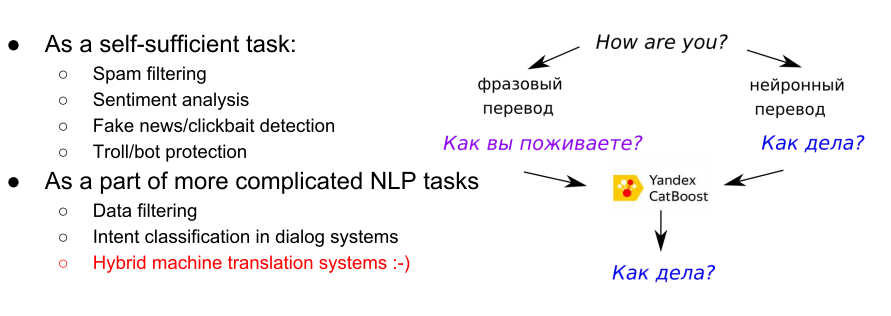
\includegraphics[width=\linewidth,keepaspectratio]{classify1}
\end{center}

{\tiny (Ref: Text Classification - Elena Voita, Yandex Research)}
\end{frame}


%%%%%%%%%%%%%%%%%%%%%%%%%%%%%%%%%%%%%%%%%%%%%%%%%%%%%%%%%%%%%%%%%%%%%%%%%%%%%%%%%%
\begin{frame}[fragile]
  \frametitle{Text classification Applications}
\begin{itemize}
\item Web pages organized into category hierarchies
\item Journal articles indexed by subject categories (e.g., the Library of Congress, MEDLINE, etc.)
\item E-mail message filtering: Spam vs. anti-palm
\item News events tracked and filtered by topics
\end{itemize}
\end{frame}

%%%%%%%%%%%%%%%%%%%%%%%%%%%%%%%%%%%%%%%%%%%%%%%%%%%%%%%%%%%%%%%%%%%%%%%%%%%%%%%%%%
\begin{frame}[fragile]
  \frametitle{News topic classification , example}
Training Data: Reuters
\begin{itemize}
\item Gold standard
\item Collection of (21,578) newswire documents. 
\item For research purposes: a standard text collection to compare systems and algorithms
\item 135 valid topics categories
\end{itemize}
\begin{center}
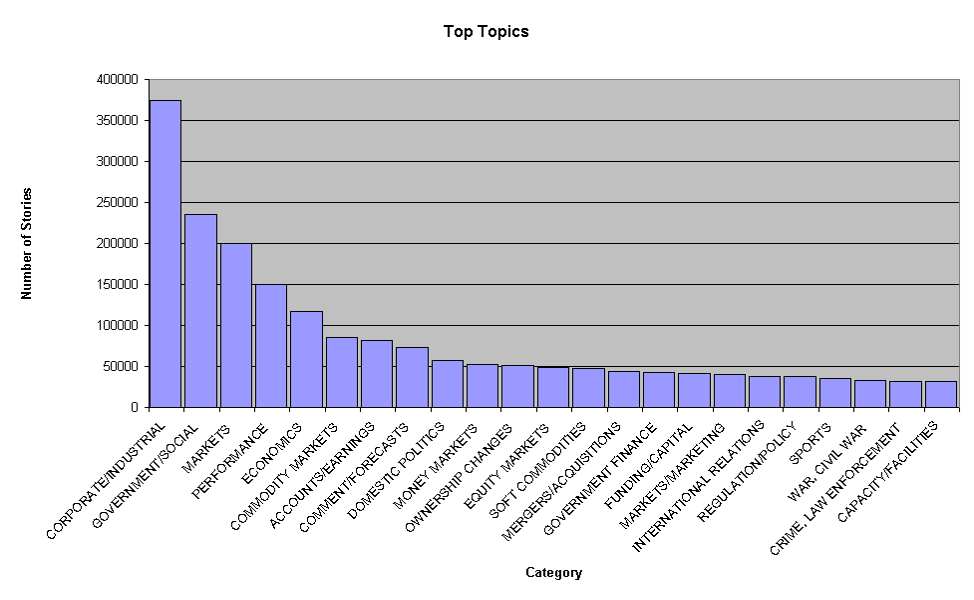
\includegraphics[width=0.8\linewidth,keepaspectratio]{class3}
\end{center}
\end{frame}

%%%%%%%%%%%%%%%%%%%%%%%%%%%%%%%%%%%%%%%%%%%%%%%%%%%%%%%%%%%%%%%%%%%%%%%%%%%%%%%%%%
\begin{frame}[fragile]
  \frametitle{Reuters Sample}
\begin{center}
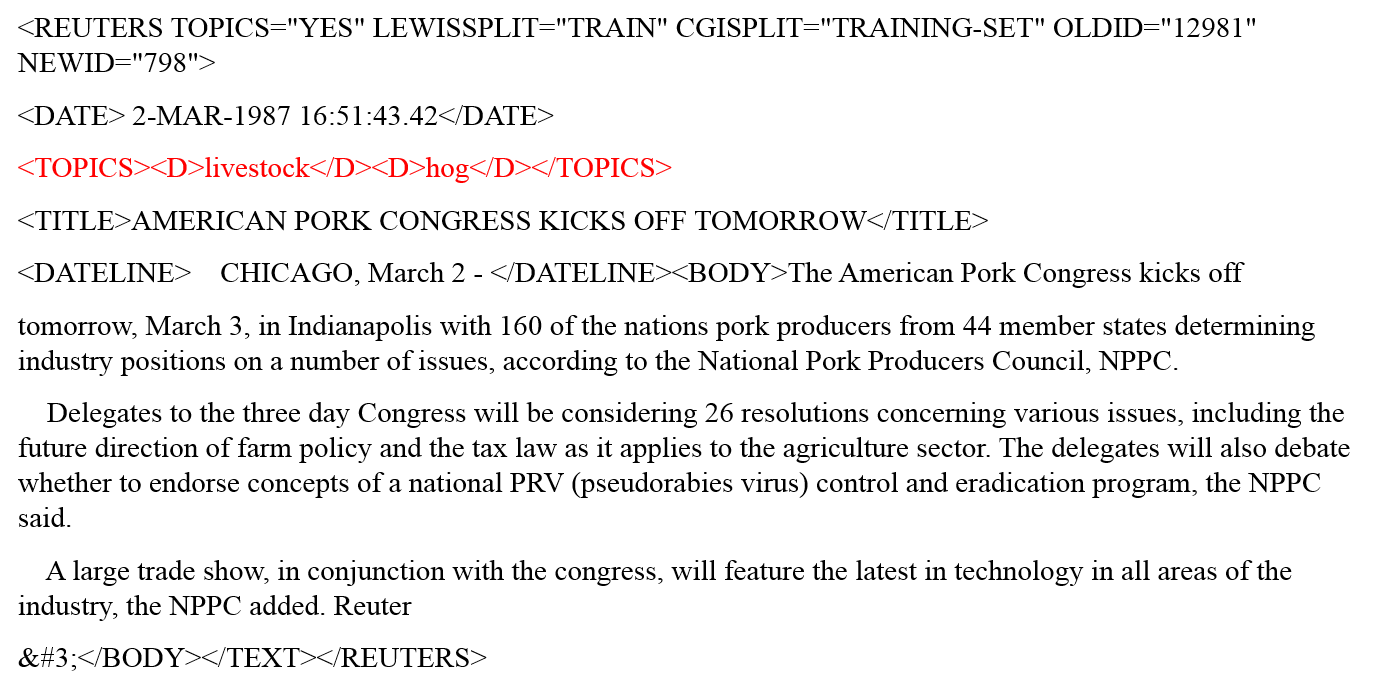
\includegraphics[width=0.8\linewidth,keepaspectratio]{class4}
\end{center}
\end{frame}

%%%%%%%%%%%%%%%%%%%%%%%%%%%%%%%%%%%%%%%%%%%%%%%%%%%%%%%%%%%%%%%%%%%%%%%%%%%%%%%%%%
\begin{frame}[fragile]
  \frametitle{How Does Text Classification Work?}
Manual and Automatic 
\begin{itemize}
\item Manual: a human annotator interprets the content of text and categorizes it accordingly. This method usually can provide quality results but it’s time-consuming and expensive. 
\item Automatic: applies machine learning, natural language processing, and other techniques to automatically classify text in a faster and more cost-effective way, but could be error-prone
\end{itemize}
\end{frame}

%%%%%%%%%%%%%%%%%%%%%%%%%%%%%%%%%%%%%%%%%%%%%%%%%%%%%%%%%%%%%%%%%%%%%%%%%%%%%%%%%%
\begin{frame}[fragile]
  \frametitle{Within Automatic}
Three different types of systems:
\begin{itemize}
\item Rule-based systems
\item Machine Learning based systems
\item Hybrid systems
\end{itemize}
\end{frame}


%%%%%%%%%%%%%%%%%%%%%%%%%%%%%%%%%%%%%%%%%%%%%%%%%%%%%%%%%%%%%%%%%%%%%%%%%%%%%%%%%%
\begin{frame}[fragile]
  \frametitle{Classification Aspects}
\begin{itemize}
\item Various issues regarding classification: Clustering vs. classification, binary vs. multi-way, flat vs. hierarchical classification, variants…
\item Introduce the steps necessary for a classification task
\begin{itemize}
\item Define classes (aka labels)
\item Label text
\item Define and extract features
\item Training and evaluation
\end{itemize}
\end{itemize}
\end{frame}


%%%%%%%%%%%%%%%%%%%%%%%%%%%%%%%%%%%%%%%%%%%%%%%%%%%%%%%%%%%%%%%%%%%%%%%%%%%%%%%%%%
\begin{frame}[fragile]
  \frametitle{What is Text Classification?}
Assign the correct class label for a given input/object In basic classification tasks, each input is considered in isolation from all other inputs, and the set of labels is defined in advance. 
\begin{center}
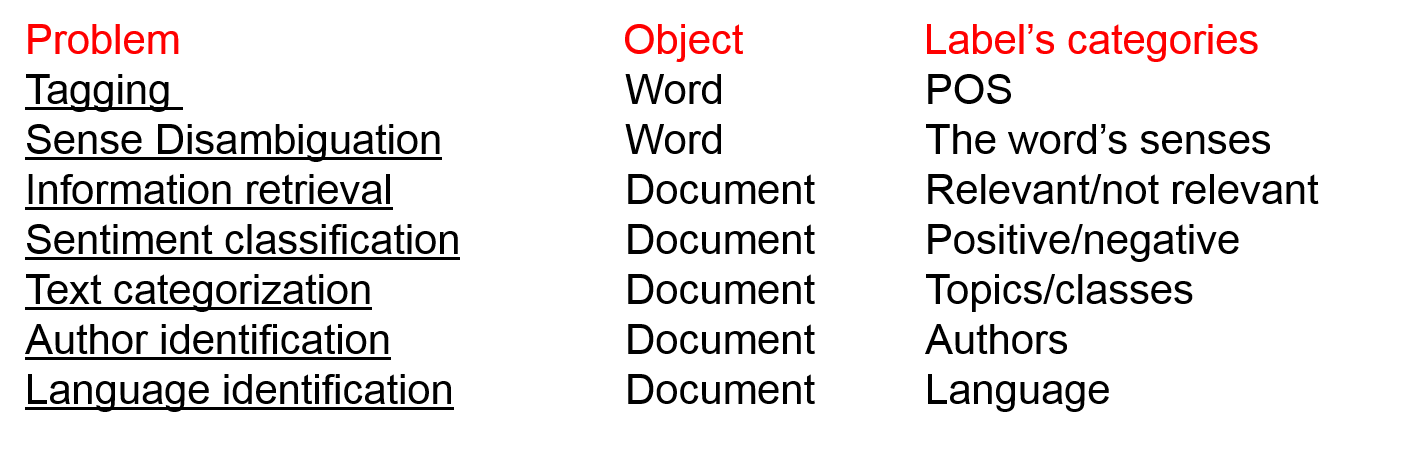
\includegraphics[width=0.8\linewidth,keepaspectratio]{class1}
\end{center}
\end{frame}

%%%%%%%%%%%%%%%%%%%%%%%%%%%%%%%%%%%%%%%%%%%%%%%%%%%%%%%%%%%%%%%%%%%%%%%%%%%%%%%%%%
\begin{frame}[fragile]
  \frametitle{Text Classification}
Classify the document into semantics topics
\begin{center}
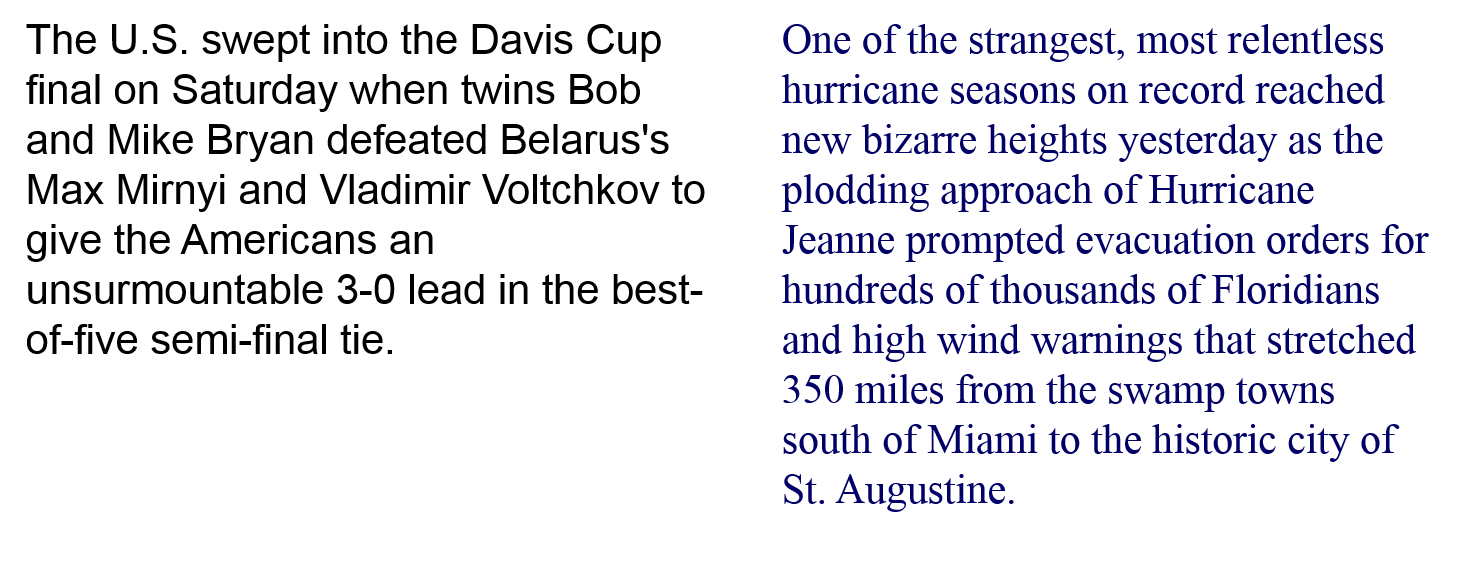
\includegraphics[width=0.8\linewidth,keepaspectratio]{class2}
\end{center}
\end{frame}

%%%%%%%%%%%%%%%%%%%%%%%%%%%%%%%%%%%%%%%%%%%%%%%%%%%%%%%%%%%%%%%%%%%%%%%%%%%%%%%%%%
\begin{frame}[fragile]
  \frametitle{Classification vs. Clustering}
\begin{itemize}
\item Classification assumes labeled data: we know how many classes there are and we have examples for each class (labeled data). 
\item Classification is supervised
\item In Clustering we don't have labeled data; we just assume that there is a natural division in the data and we may not know how many divisions (clusters) there are
\item Clustering is unsupervised
\end{itemize}
\end{frame}

%%%%%%%%%%%%%%%%%%%%%%%%%%%%%%%%%%%%%%%%%%%%%%%%%%%%%%%%%%%%%%%%%%%%%%%%%%%%%%%%%%
\begin{frame}[fragile]
  \frametitle{Supervised classification}
A classifier is called supervised if it is built based on training corpora containing the correct label for each input. 

\begin{center}
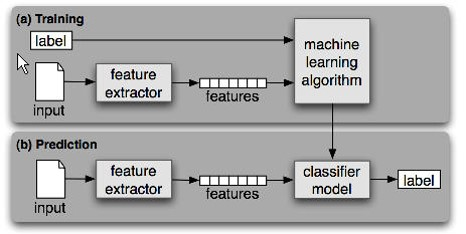
\includegraphics[width=\linewidth,keepaspectratio]{class5}
\end{center}
\end{frame}

%%%%%%%%%%%%%%%%%%%%%%%%%%%%%%%%%%%%%%%%%%%%%%%%%%%%%%%%%%%%%%%%%%%%%%%%%%%%%%%%%%
\begin{frame}[fragile]
  \frametitle{Text classification in general}
\begin{center}
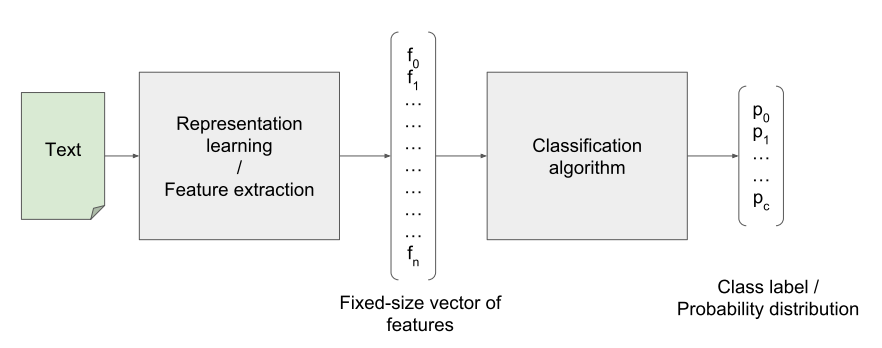
\includegraphics[width=\linewidth,keepaspectratio]{classify2}
\end{center}

{\tiny (Ref: Text Classification - Elena Voita, Yandex Research)}
\end{frame}

%%%%%%%%%%%%%%%%%%%%%%%%%%%%%%%%%%%%%%%%%%%%%%%%%%%%%%%%%%%%%%%%%%%%%%%%%%%%%%%%%%
\begin{frame}[fragile]
  \frametitle{Labels}
\begin{itemize}
\item Binary classification: spam filtering/sentiment analysis
\item Multi-class classification: categorization of goods
\item  Multi-label classification: \#hashtag prediction
\end{itemize}
\end{frame}


%%%%%%%%%%%%%%%%%%%%%%%%%%%%%%%%%%%%%%%%%%%%%%%%%%%%%%%%%%%%%%%%%%%%%%%%%%%%%%%%%%
\begin{frame}[fragile]
  \frametitle{Training}
\begin{itemize}
\item Adaptation of the classifier to the data
\item Usually the classifier is defined by a set of parameters
\item Training is the procedure for finding a ``good'' set of parameters
\item Goodness is determined by an optimization criterion such as misclassification rate
\item Some classifiers are guaranteed to find the optimal set of parameters
\end{itemize}
\end{frame}


%%%%%%%%%%%%%%%%%%%%%%%%%%%%%%%%%%%%%%%%%%%%%%%%%%%%%%%%%%%%%%%%%%%%%%%%%%%%%%%%%%
\begin{frame}[fragile]
  \frametitle{Algorithms for Classification}
\begin{itemize}
\item It's possible to treat these learning methods as black boxes. 
\item But there's a lot to be learned from taking a closer look 
\item An understanding of these methods can help guide our choice for the appropriate learning method (binary or multi-class for example)
\item Binary classification: Linear and not linear
\item Multi-Class classification: Linear and not linear
\end{itemize}
\end{frame}

%%%%%%%%%%%%%%%%%%%%%%%%%%%%%%%%%%%%%%%%%%%%%%%%%%%%%%%%%%%%%%%%%%%%%%%%%%%%%%%%%%
\begin{frame}[fragile]
  \frametitle{Methods}
\begin{itemize}
\item Linear Models:
\begin{itemize}
\item Perceptron \& Winnow (neural networks)
\item Large margin classifier 
\item Support Vector Machine (SVM)
\end{itemize}
\item Probabilistic models:
\begin{itemize}
\item Naive Bayes
\item Maximum Entropy Models
\end{itemize}
\item Decision Models: Decision Trees
\item Instance-based methods: Nearest neighbor
\end{itemize}
\end{frame}

%%%%%%%%%%%%%%%%%%%%%%%%%%%%%%%%%%%%%%%%%%%%%%%%%%%%%%%%%%%%%%%%%%%%%%%%%%%%%%%%%%
\begin{frame}[fragile]
  \frametitle{(Linear) Classification}
Choose the classier with the lower rate of misclassification
\begin{center}
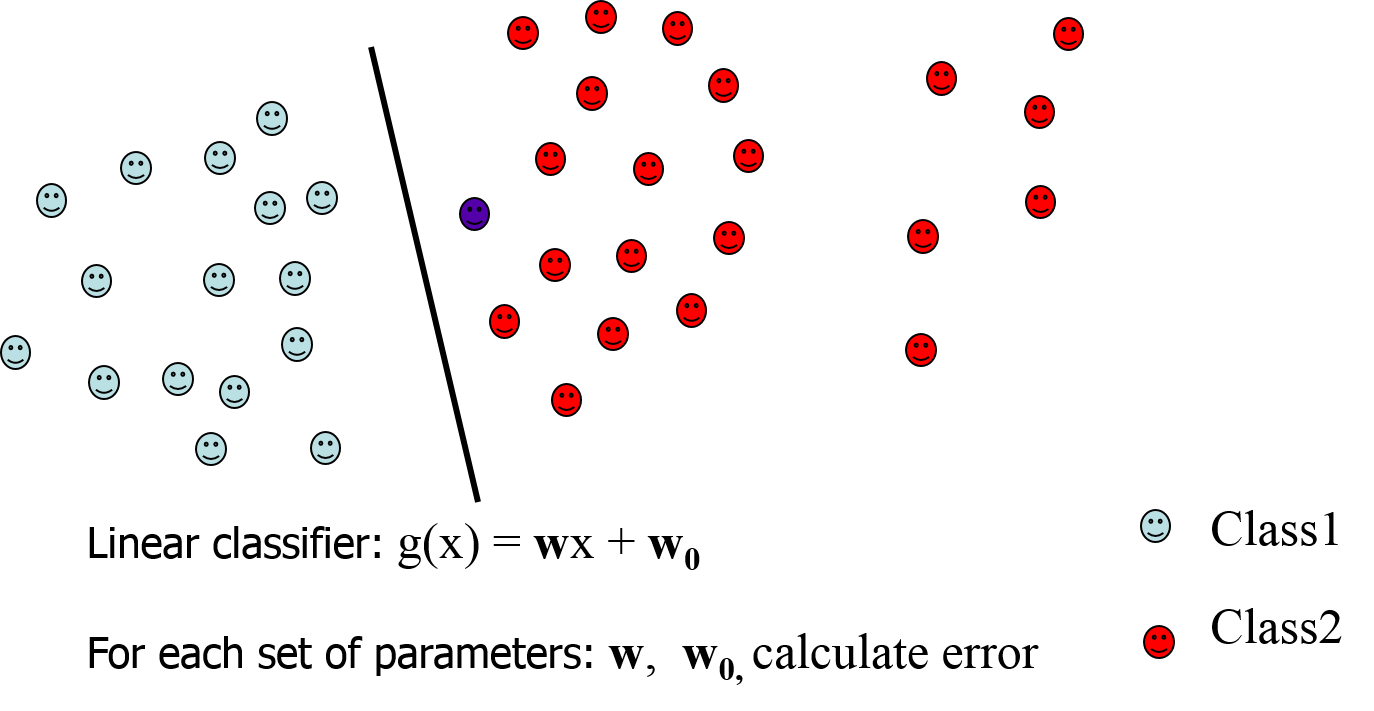
\includegraphics[width=\linewidth,keepaspectratio]{class6}
\end{center}
\end{frame}

%%%%%%%%%%%%%%%%%%%%%%%%%%%%%%%%%%%%%%%%%%%%%%%%%%%%%%%%%%%%%%%%%%%%%%%%%%%%%%%%%%
\begin{frame}[fragile]
  \frametitle{Non linearly separable data}
\begin{center}
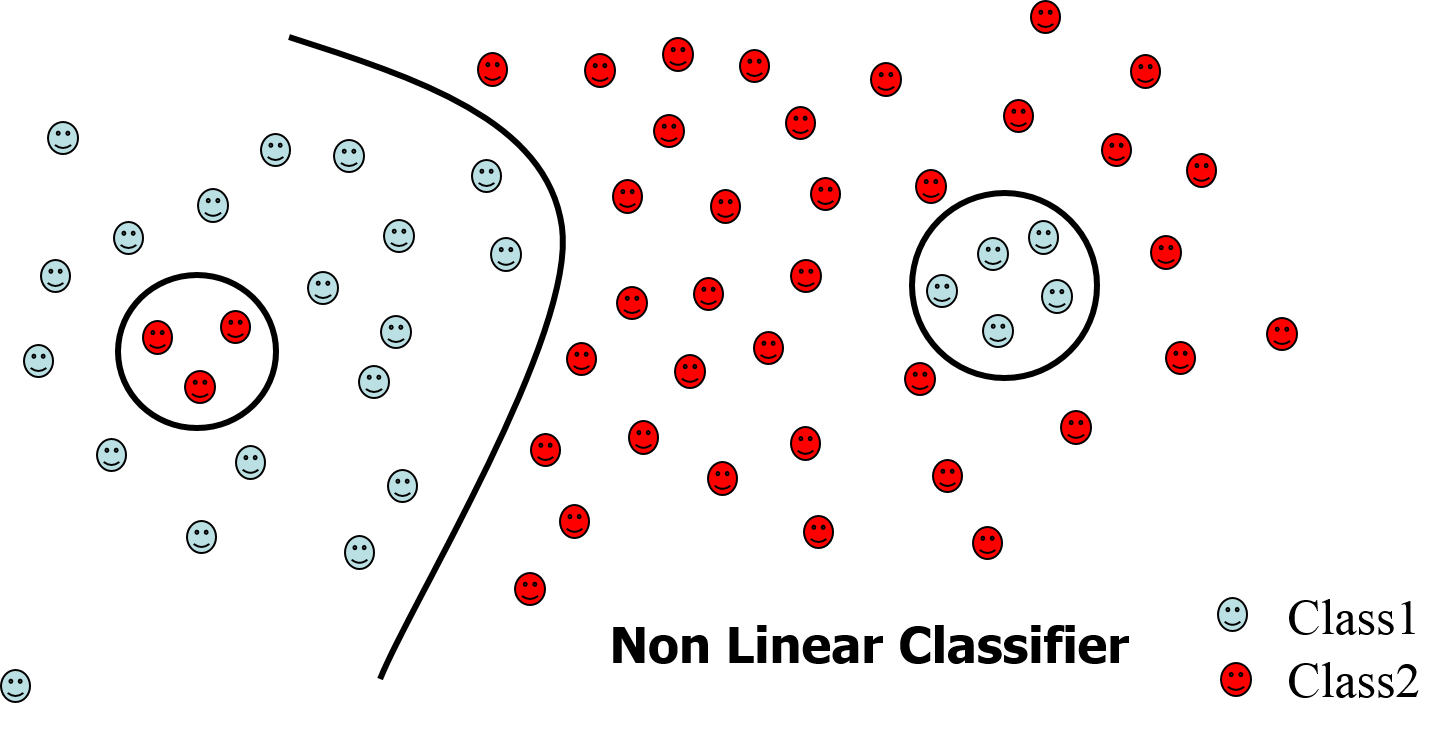
\includegraphics[width=\linewidth,keepaspectratio]{class13}
\end{center}
\end{frame}

%%%%%%%%%%%%%%%%%%%%%%%%%%%%%%%%%%%%%%%%%%%%%%%%%%%%%%%%%%%%%%%%%%%%%%%%%%%%%%%%%%
\begin{frame}[fragile]
  \frametitle{Multi-class classification}
\begin{center}
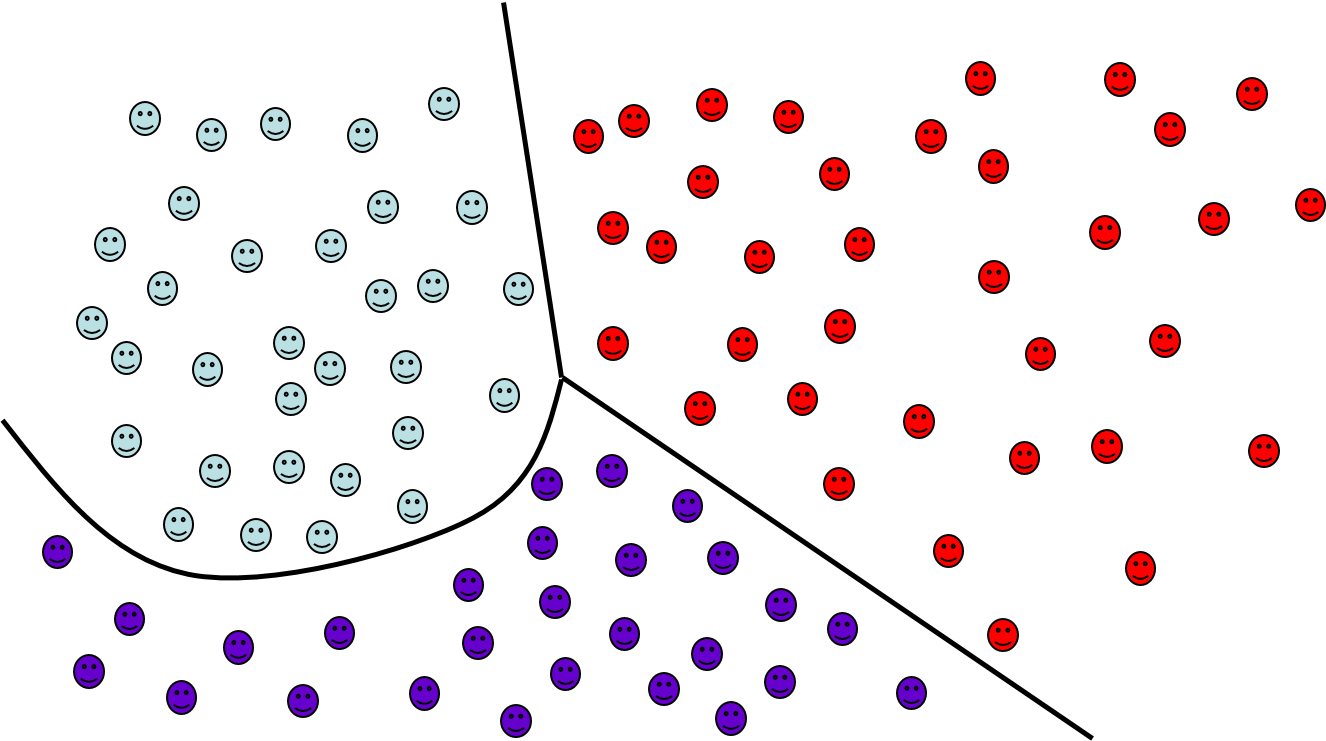
\includegraphics[width=\linewidth,keepaspectratio]{class14}
\end{center}
\end{frame}

%%%%%%%%%%%%%%%%%%%%%%%%%%%%%%%%%%%%%%%%%%%%%%%%%%%%%%%%%%%%%%%%%%%%%%%%%%%%%%%%%%
\begin{frame}[fragile]
  \frametitle{Linear, parallel class separators (ex: Decision Trees)}
\begin{center}
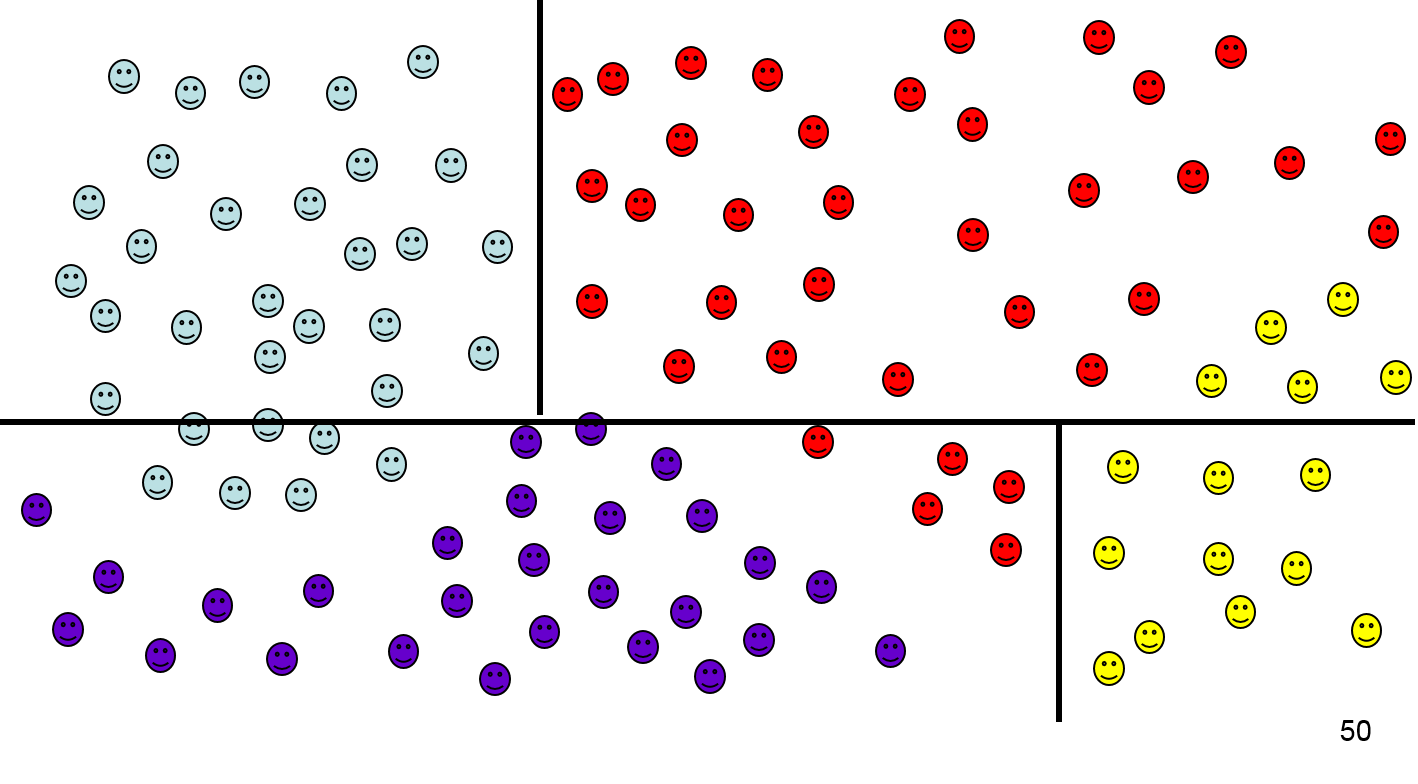
\includegraphics[width=\linewidth,keepaspectratio]{class15}
\end{center}
\end{frame}

%%%%%%%%%%%%%%%%%%%%%%%%%%%%%%%%%%%%%%%%%%%%%%%%%%%%%%%%%%%%%%%%%%%%%%%%%%%%%%%%%%
\begin{frame}[fragile]
  \frametitle{Non Linear (ex: k Nearest Neighbor)}
\begin{center}
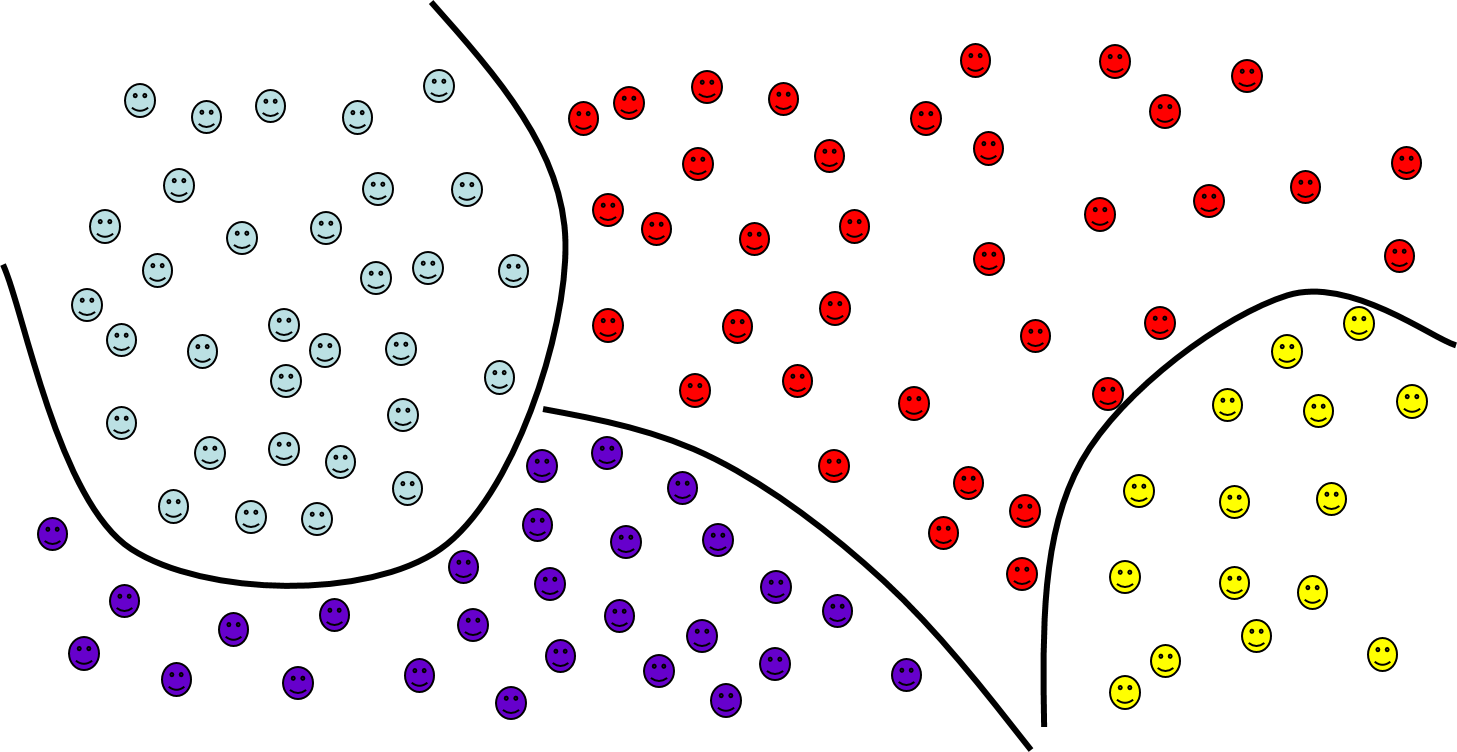
\includegraphics[width=\linewidth,keepaspectratio]{class16}
\end{center}
\end{frame}

%%%%%%%%%%%%%%%%%%%%%%%%%%%%%%%%%%%%%%%%%%%%%%%%%%%%%%%%%%%%%%%%%%%%%%%%%%%%%%%%%%
\begin{frame}[fragile]
  \frametitle{Naïve Bayes}
More powerful that Decision Trees
\begin{center}
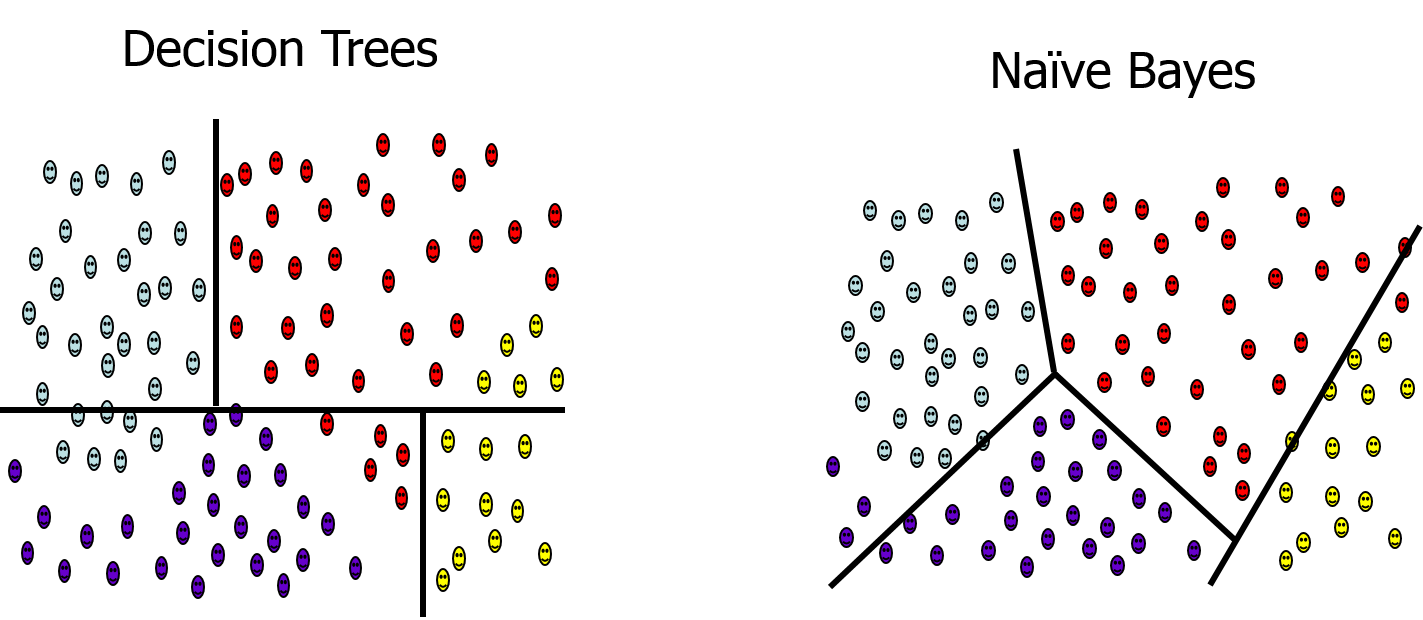
\includegraphics[width=\linewidth,keepaspectratio]{class17}
\end{center}
\end{frame}

%%%%%%%%%%%%%%%%%%%%%%%%%%%%%%%%%%%%%%%%%%%%%%%%%%%%%%%%%%%%%%%%%%%%%%%%%%%%%%%%%%
\begin{frame}[fragile]
  \frametitle{Testing \& Evaluation}
\begin{itemize}
\item After choosing the parameters of the classifiers (i.e. after training it) we need to test how well it's doing on a test set (not included in the training set)
\item How trustworthy the model is
\item Evaluation can also be an effective tool for guiding us in making future improvements to the model. 

\end{itemize}
\end{frame}

%%%%%%%%%%%%%%%%%%%%%%%%%%%%%%%%%%%%%%%%%%%%%%%%%%%%%%%%%%%%%%%%%%%%%%%%%%%%%%%%%%
\begin{frame}[fragile]
  \frametitle{Accuracy}
\begin{itemize}
\item The simplest metric: accuracy, measures the percentage of inputs in the test set that the classifier correctly labeled. 
\item For example, a spam classifier that predicts correctly spam 60 times in an test set containing 80 email would have an accuracy of 60/80 = 75\%. 
\item Important to take into consideration the frequencies of the individual class labels 
\item If only 1/100 is spam, an accuracy of 90\% is bad
\item If 1/2 is spam, accuracy of 90\% is good
\item This is also why we use precision \& recall and F-measure
\item Important: compare with fair baselines 


\end{itemize}
\end{frame}

%%%%%%%%%%%%%%%%%%%%%%%%%%%%%%%%%%%%%%%%%%%%%%%%%%%%%%%%%%%%%%%%%%%%%%%%%%%%%%%%%%
\begin{frame}[fragile]
  \frametitle{Evaluating classifiers}
Contingency table for the evaluation of a binary classifier
\begin{center}
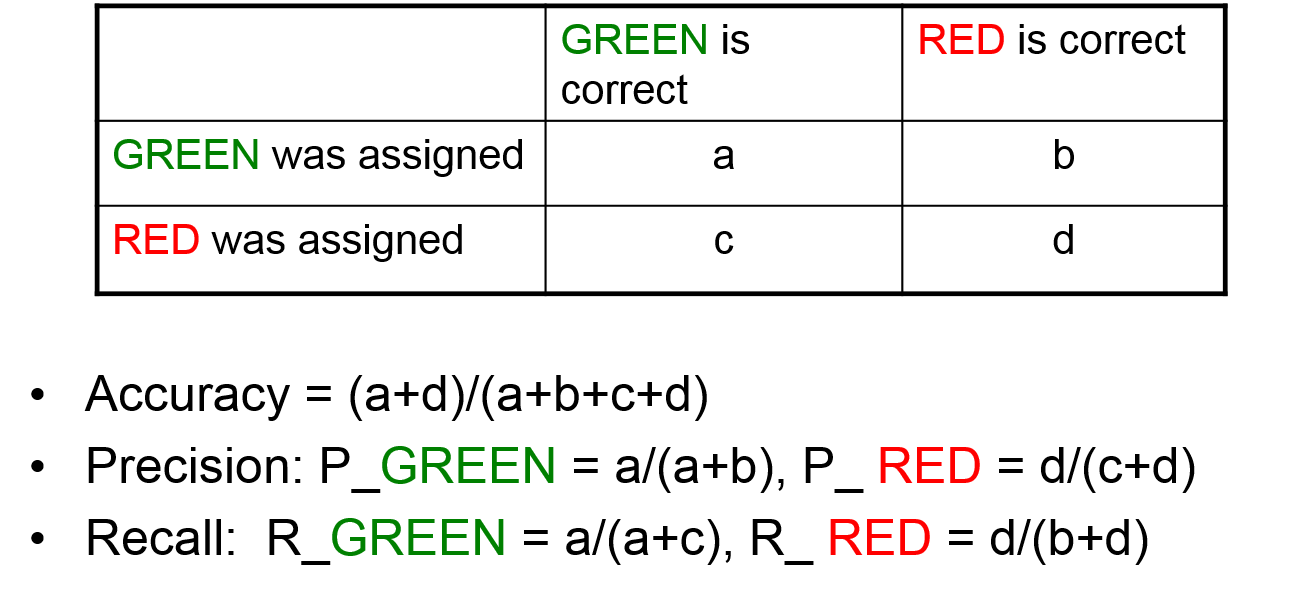
\includegraphics[width=0.7\linewidth,keepaspectratio]{class7}
\end{center}
\end{frame}



%%%%%%%%%%%%%%%%%%%%%%%%%%%%%%%%%%%%%%%%%%%%%%%%%%%%%%%%%%%%%%%%%%%%%%%%%%%%%%%%%%
\begin{frame}[fragile]
  \frametitle{Representation of Objects}
\begin{itemize}
\item Each object to be classified is represented as a pair (x, y):
\begin{itemize}
\item where x is a description of the object
\item where y is a label
\end{itemize}
\item Success or failure of a machine learning classifier often depends on choosing good descriptions of objects
\begin{itemize}
\item the choice of description can also be viewed as a learning problem (feature selections)
\item but good human intuitions are often needed here
\end{itemize}
\end{itemize}
\end{frame}


%%%%%%%%%%%%%%%%%%%%%%%%%%%%%%%%%%%%%%%%%%%%%%%%%%%%%%%%%%%%%%%%%%%%%%%%%%%%%%%%%%
\begin{frame}[fragile]
  \frametitle{Feature Engineering}
  
  As for many ML tasks, it is possible to generate useful features by hands
  
\begin{itemize}
\item General statistics: text length, text length variance, etc
\item Domain or Linguistic dictionaries
\item POS, NER tags
\item Topic Models as features
\item Ad-hoc features: e.g. number of emojis
\end{itemize}

And also, embeddings (bow, tfidf, distributed vectors, etc) \ldots
\end{frame} 

%%%%%%%%%%%%%%%%%%%%%%%%%%%%%%%%%%%%%%%%%%%%%%%%%%%%%%%%%%%%%%%%%%%%%%%%%%%%%%%%%%
\begin{frame}[fragile]
  \frametitle{Improving Text Classification Models}
  
Practical tips:
  
\begin{itemize}
\item Text Cleaning : text cleaning can help to reducue the noise present in text data in the form of stopwords, punctuations marks, suffix variations etc.
\item More intuitive domain and NLP features along with embedding vectors
\item Hyperparamter Tuning in modelling : Tuning the paramters is an important step, a number of parameters such as tree length, leafs, network paramters etc can be fine tuned to get a best fit model.
\item Ensemble Models : Stacking different models and blending their outputs can help to further improve the results.
\end{itemize}
\end{frame} 

%%%%%%%%%%%%%%%%%%%%%%%%%%%%%%%%%%%%%%%%%%%%%%%%%%%%%%%%%%%%%%%%%%%%%%%%%%%%%%%%%%
\begin{frame}[fragile]
  \frametitle{Summary}
\begin{itemize}
\item We discussed about how to prepare a text dataset 
\item Perform different types of feature engineering like Count Vector/TF-IDF/ Word Embedding/ Topic Modelling and basic text features, 
\item Finally trained a variety of classifiers like Naive Bayes/ Logistic regression/ SVM
\end{itemize}

\end{frame} 


